\documentclass[11pt,a4paper]{report}
\usepackage[tmargin=1cm,rmargin=1in,lmargin=1in,margin=0.2in,bmargin=1cm,footskip=.2in]{geometry}
\title{REAL112-1 24H - Matematikk\\Obligatorisk innlevering 5}
\author{Casper Eide Özdemir-Børretzen}
\date{}
\makeatletter
\newcommand{\institle}{\@title}
\newcommand{\insauthor}{\@author}
\newcommand{\insdate}{\@date}
\makeatother

% % % % % % % % % % % % % % % % % % % % % % % % % % % % % % % % % % % % % % % % 

\usepackage{setspace}
\usepackage{empheq}
\usepackage{nicefrac}
\usepackage{graphicx}            % Images
\usepackage{gensymb}             % Degree symbol
\usepackage{listings}            % Code
\usepackage{ulem}                % Double underline
\usepackage{amssymb}             %
\usepackage{pdfpages}            % Insert pdf pages
\usepackage{enumitem}            % Lists
\usepackage{titlesec}            %
\usepackage[T1]{fontenc}         %
\usepackage[utf8]{inputenc}      %
\usepackage[fleqn]{amsmath}      %
\usepackage[makeroom]{cancel}    %
\setstretch{1.5}
\setlength{\parindent}{0pt}
\titlespacing*{\subsection}{0cm}{2cm}{0.5cm}
\lstset{
aboveskip=0cm,
belowskip=0cm,
showstringspaces=false,
columns=flexible,
basicstyle={\scriptsize\ttfamily},
breaklines=true,
breakatwhitespace=true,
tabsize=4,
inputencoding = utf8,  % Input encoding
extendedchars = true,  % Extended ASCII
literate      =        % Support additional characters
{á}{{\'a}}1  {é}{{\'e}}1  {í}{{\'i}}1 {ó}{{\'o}}1  {ú}{{\'u}}1
{Á}{{\'A}}1  {É}{{\'E}}1  {Í}{{\'I}}1 {Ó}{{\'O}}1  {Ú}{{\'U}}1
{à}{{\`a}}1  {è}{{\`e}}1  {ì}{{\`i}}1 {ò}{{\`o}}1  {ù}{{\`u}}1
{À}{{\`A}}1  {È}{{\`E}}1  {Ì}{{\`I}}1 {Ò}{{\`O}}1  {Ù}{{\`U}}1
{ä}{{\"a}}1  {ë}{{\"e}}1  {ï}{{\"i}}1 {ö}{{\"o}}1  {ü}{{\"u}}1
{Ä}{{\"A}}1  {Ë}{{\"E}}1  {Ï}{{\"I}}1 {Ö}{{\"O}}1  {Ü}{{\"U}}1
{â}{{\^a}}1  {ê}{{\^e}}1  {î}{{\^i}}1 {ô}{{\^o}}1  {û}{{\^u}}1
{Â}{{\^A}}1  {Ê}{{\^E}}1  {Î}{{\^I}}1 {Ô}{{\^O}}1  {Û}{{\^U}}1
{œ}{{\oe}}1  {Œ}{{\OE}}1  {æ}{{\ae}}1 {Æ}{{\AE}}1  {ß}{{\ss}}1
{ẞ}{{\SS}}1  {ç}{{\c{c}}}1 {Ç}{{\c{C}}}1 {ø}{{\o}}1  {Ø}{{\O}}1
{å}{{\aa}}1  {Å}{{\AA}}1  {ã}{{\~a}}1  {õ}{{\~o}}1 {Ã}{{\~A}}1
{Õ}{{\~O}}1  {ñ}{{\~n}}1  {Ñ}{{\~N}}1  {¿}{{?`}}1  {¡}{{!`}}1
{„}{\quotedblbase}1 {“}{\textquotedblleft}1 {–}{$-$}1
{°}{{\textdegree}}1 {º}{{\textordmasculine}}1 {ª}{{\textordfeminine}}1
{£}{{\pounds}}1  {©}{{\copyright}}1  {®}{{\textregistered}}1
{«}{{\guillemotleft}}1  {»}{{\guillemotright}}1  {Ð}{{\DH}}1  {ð}{{\dh}}1
{Ý}{{\'Y}}1    {ý}{{\'y}}1    {Þ}{{\TH}}1    {þ}{{\th}}1    {Ă}{{\u{A}}}1
{ă}{{\u{a}}}1  {Ą}{{\k{A}}}1  {ą}{{\k{a}}}1  {Ć}{{\'C}}1    {ć}{{\'c}}1
{Č}{{\v{C}}}1  {č}{{\v{c}}}1  {Ď}{{\v{D}}}1  {ď}{{\v{d}}}1  {Đ}{{\DJ}}1
{đ}{{\dj}}1    {Ė}{{\.{E}}}1  {ė}{{\.{e}}}1  {Ę}{{\k{E}}}1  {ę}{{\k{e}}}1
{Ě}{{\v{E}}}1  {ě}{{\v{e}}}1  {Ğ}{{\u{G}}}1  {ğ}{{\u{g}}}1  {Ĩ}{{\~I}}1
{ĩ}{{\~\i}}1   {Į}{{\k{I}}}1  {į}{{\k{i}}}1  {İ}{{\.{I}}}1  {ı}{{\i}}1
{Ĺ}{{\'L}}1    {ĺ}{{\'l}}1    {Ľ}{{\v{L}}}1  {ľ}{{\v{l}}}1  {Ł}{{\L{}}}1
{ł}{{\l{}}}1   {Ń}{{\'N}}1    {ń}{{\'n}}1    {Ň}{{\v{N}}}1  {ň}{{\v{n}}}1
{Ő}{{\H{O}}}1  {ő}{{\H{o}}}1  {Ŕ}{{\'{R}}}1  {ŕ}{{\'{r}}}1  {Ř}{{\v{R}}}1
{ř}{{\v{r}}}1  {Ś}{{\'S}}1    {ś}{{\'s}}1    {Ş}{{\c{S}}}1  {ş}{{\c{s}}}1
{Š}{{\v{S}}}1  {š}{{\v{s}}}1  {Ť}{{\v{T}}}1  {ť}{{\v{t}}}1  {Ũ}{{\~U}}1
{ũ}{{\~u}}1    {Ū}{{\={U}}}1  {ū}{{\={u}}}1  {Ů}{{\r{U}}}1  {ů}{{\r{u}}}1
{Ű}{{\H{U}}}1  {ű}{{\H{u}}}1  {Ų}{{\k{U}}}1  {ų}{{\k{u}}}1  {Ź}{{\'Z}}1
{ź}{{\'z}}1    {Ż}{{\.Z}}1    {ż}{{\.z}}1    {Ž}{{\v{Z}}}1  {ž}{{\v{z}}}1
}

% % % % % % % % % % % % % % % % % % % % % % % % % % % % % % % % % % % % % % % % 

\newcommand{\m}{\cdot}
\newcommand{\opgd}[1]{\item[#1)]}
\newcommand{\opg}[1]{\subsection*{Oppgave #1}}
\newcommand{\enkelsvaralign}[1]{\makebox[0pt][l]{\uuline{\phantom{$#1$}}}#1}
\newcommand{\svaralign}[2]{\makebox[0pt][l]{\uuline{\phantom{$#1 #2$}}}#1 &#2}

% % % % % % % % % % % % % % % % % % % % % % % % % % % % % % % % % % % % % % % % 

\begin{document}
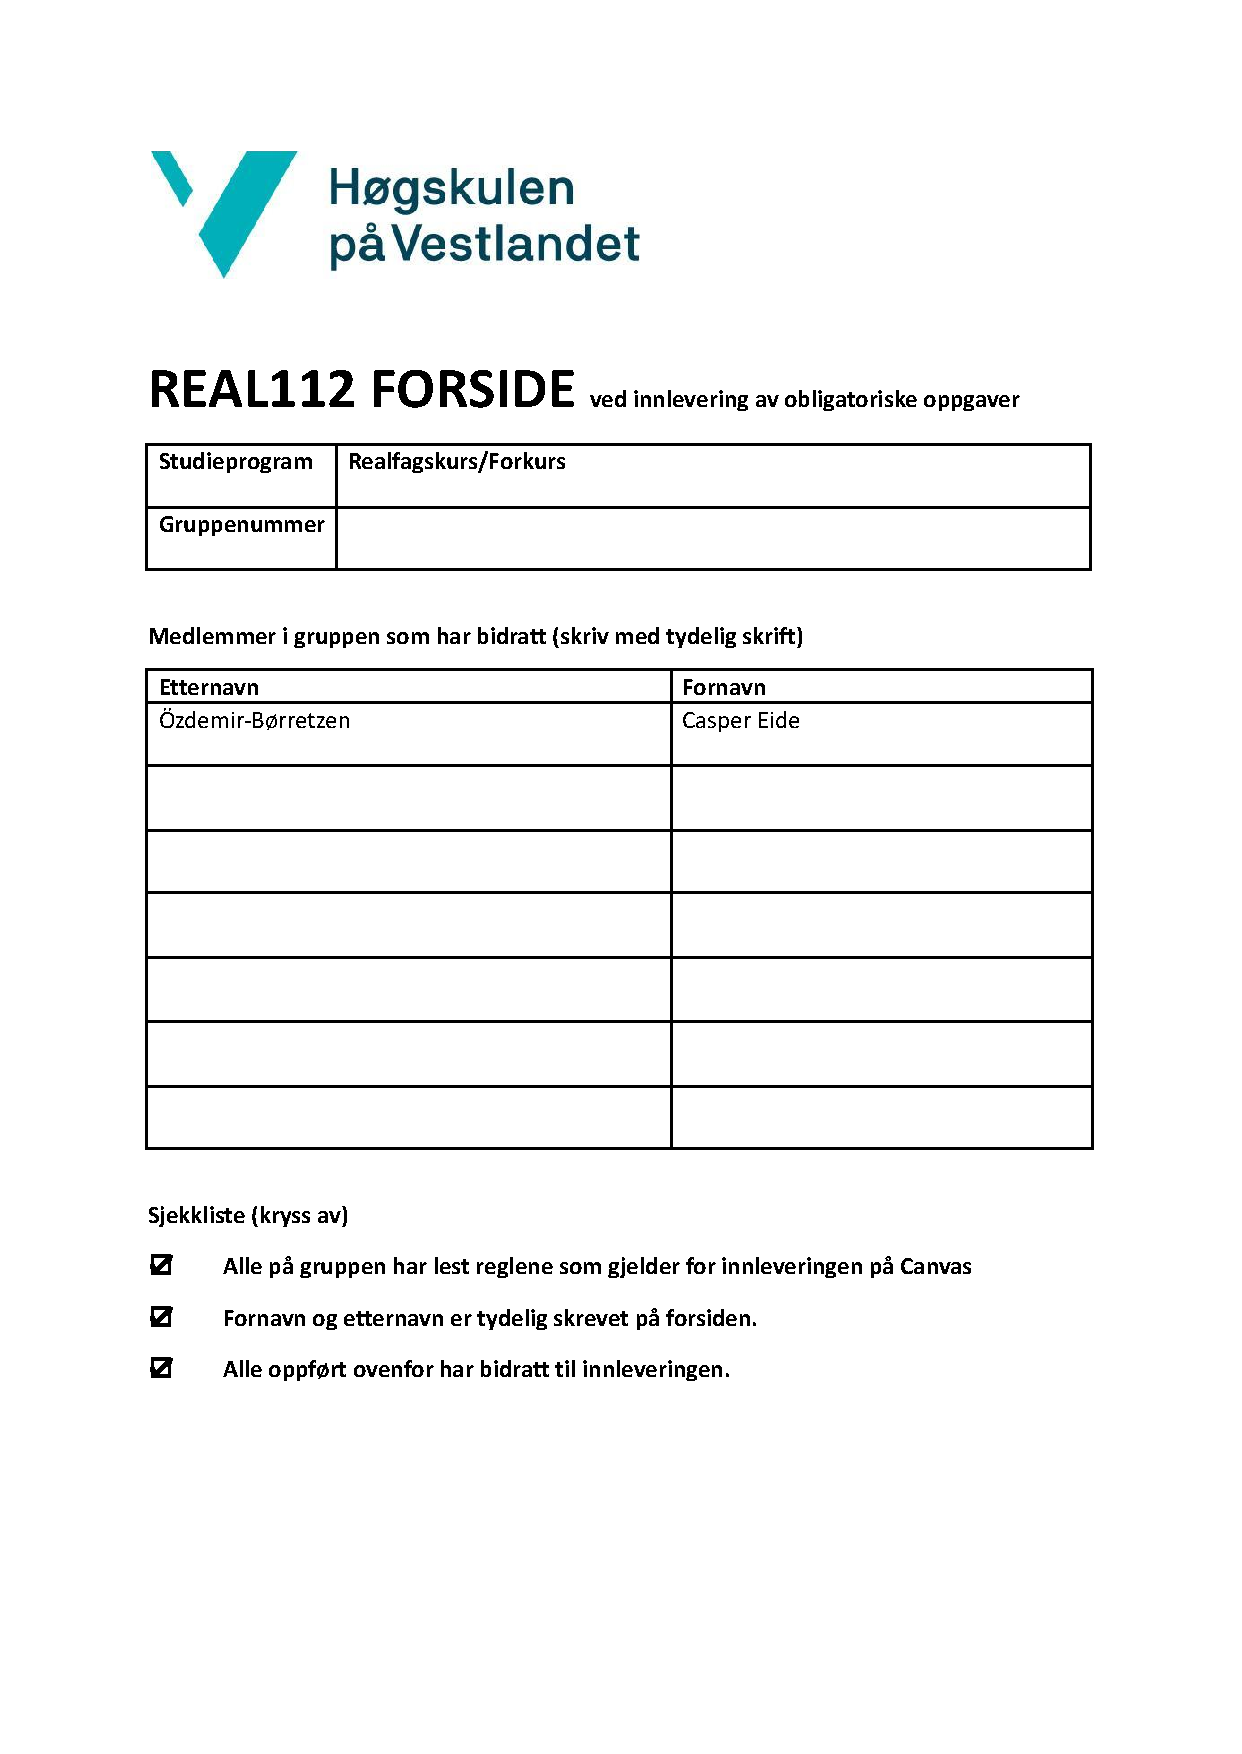
\includepdf[pages={1}]{real112-forside.pdf}

% % % % % % % % % % % % % % % % % % % % % % % % % % % % % % % % % % % % % % % % 

\opg{1}
\begin{enumerate}[leftmargin=*,itemsep=0.75cm,labelsep=1.5em,label=\alph*)]
\opgd{a}
\begin{align*}
&v = 63,5\ \degree\\
&\tab v = \frac{AB}{OA}\\
&AB = \tan v \cdot OA &\text{der $OA = 1$ i enhetssirkelen}\\
&AB = \tan 63,5 \degree = \uuline{2,005689708}
\end{align*}
\end{enumerate}

% % % % % % % % % % % % % % % % % % % % % % % % % % % % % % % % % % % % % % % % 

\opg{2}
\begin{enumerate}[leftmargin=*,itemsep=0.75cm,labelsep=1.5em,label=\alph*)]
\opgd{a}
\begin{align*}
&(2 \cdot \sin x - \sqrt{3}) (2 \cdot \cos x + 3) = 0, x \in [-\pi, \pi]\\
&4 \cdot \sin x \cdot cos x + 6 \sin x - 2 \sqrt{3} \cdot cos x - 3 \sqrt{3} = 0 &&(1)\\
&\boxed{sin^2 x + cos^2 x = 1} \\
&\cos^2 x = 1 - sin^2 x &&(2)\\
&\text{$(2)$ inn i $(1)$:}\\
&4 \cdot \sin x \cdot (1 - \sin^2 x) + 6 \sin x - 2 \sqrt{3} \cdot (1 - \sin^2 x) - 3 \sqrt{3} = 0\\
&4 \cdot \sin x - 4 \cdot \sin^3 x + 6 \sin x - 2 \sqrt{3} + 2 \sqrt{3} \sin^2 x - 3 \sqrt{3} = 0\\
&4 \cdot \sin x + 6 \sin x + 2 \sqrt{3} \sin^2 x - 4 \sin^3 x - 3 \sqrt{3} - 2 \sqrt{3} = 0\\
&10 \sin x + 2 \sqrt{3} \sin^2 x - 4 \sqin^3 x - 5 \sqrt{3} = 0\\
&2 \sin x (5 - 2 \sin^2 x) - \sqrt{3} (5 - 2 \sin^2) = 0\\
&(5 - 2 \sin^2 x) (2 \sin x - \sqrt{3}) = 0\\
&2 \sin x - \sqrt{3} = 0    &&\lor &&5 - 2 \sin^2 x = 0\\
&\sin x = \frac{\sqrt{3}}{2} &&\lor &&\sin x = \sqrt{\frac{5}{2}}\\
&x = \sin^{-1}(\frac{\sqrt{3}}{2}) &&\lor &&\text{$\sin x$ er over $1$, så $\sin^{-1}$}\\
&x = \uuline{\frac{\pi}{3}} && &&\text{gir ingen løsning.}
\end{align*}
\end{enumerate}

\newpage
\opg{2}
\begin{enumerate}[leftmargin=*,itemsep=0.75cm,labelsep=1.5em,label=\alph*)]
\opgd{b}
\begin{align*}
&6 \sin^2 x + \sin x - 1 = 0, x \in [0, 2 \pi]\\
&\boxed{ax^2 + bx + c = 0} \rightarrow \boxed{a \cdot c = d \cdot e \ \land \ b = d + e} \rightarrow \boxed{ax^2 + dx + ex + c = 0}\\
&a = 6 \ \ \ \ b = 1 \ \ \ \ c = -1 \ \ \ \ d = -2 \ \ \ \ e = 3\\
&6 \sin^2 x + 3 \sin x - 2 \sin x - 1 = 0\\
&3 \sin x (2 \sin x + 1) - 1 (2 \sin x + 1) = 0\\
&(2 \sin x + 1) (3 \sin x - 1) = 0\\
&2 \sin x + 1 = 0\\
&\sin x = - \frac{1}{2}\\
&x = \frac{12 \pi}{6} - \frac{\pi}{6} = \frac{11 \pi}{6} \ \ \ \ \lor \ \ \ \ x = \frac{6 \pi}{6} + \frac{\pi}{6} = \frac{7 \pi}{6}\\
&3 \sin x - 1 = 0\\
&\sin x = \frac{1}{3}\\
&x = \frac{1}{3} \ \ \ \ \lor \ \ \ \ x = \pi - \frac{1}{3}\\[0.2cm]
&x = \uuline{\frac{1}{3}} \ \ \ \ \lor \ \ \ \ x = \uuline{\pi - \frac{1}{3}} \ \ \ \ \lor \ \ \ \ x = \uuline{\frac{7 \pi}{6}} \ \ \ \ \lor \ \ \ \ x = \uuline{\frac{11 \pi}{6}}
\end{align*}
\end{enumerate}

% % % % % % % % % % % % % % % % % % % % % % % % % % % % % % % % % % % % % % % % 

\newpage
\opg{3}
\begin{enumerate}[leftmargin=*,itemsep=0.75cm,labelsep=1.5em,label=\alph*)]
\item[]
\begin{align*}
&f(x) = \sqrt{2} + 2 \sin (\pi x - \frac{\pi}{4}), x \in [0, 4]&&\\
&\boxed{f(x) = a \sin (kx + c) + d}&&\\
&a = 2\\
&k = \pi\\
&c = - \frac{\pi}{4}\\
&d = \sqrt{2}\\
&p = \frac{2 \pi}{k} = \frac{2 \pi}{\pi} = 2&&\\
&x_0 = - \frac{c}{k} = - \frac{-\frac{\pi}{4}}{\pi} = \frac{\cancel{\pi}}{4} \cdot \frac{1}{\cancel{\pi}} = \frac{1}{4}
\end{align*}
\opgd{a}
Maksimalverdien for $f(x)$ er ved $\sin(\pi x - \frac{\pi}{4}) = 1$ som gir $\sqrt{2} + 2 \cdot 1 = \sqrt{2} + 2$\\
\uuline{Påstanden er feil.}
\opgd{b}
Amplituden er $|a| = 2$\\
\uuline{Påstanden er riktig.}
\opgd{c}
Likevektslinja er $d = \sqrt{2}$\\
\uuline{Påstanden er feil.}
\opgd{d}
Perioden er $p = 2$\\
\uuline{Påstanden er feil.}
\end{enumerate}

% % % % % % % % % % % % % % % % % % % % % % % % % % % % % % % % % % % % % % % % 

\newpage
\opg{4}
\begin{enumerate}[leftmargin=*,itemsep=0.75cm,labelsep=1.5em,label=\alph*)]
\item[]
\begin{align*}
&f(x) = \sqrt{2} + 2 \sin (\pi x - \frac{\pi}{4}), x \in [0, 4]\\
&f(x) = 0\\
&\sqrt{2} + 2 \sin (\pi x - \frac{\pi}{4})\\
&\sin (\pi x \frac{\pi}{4}) = \frac{\sqrt{2}}{2}\\
&\sin^{-1} (-\frac{\sqrt{2}}{2}) = -\frac{\pi}{4}\\
&v = \pi \cdot x - \frac{\pi}{4}\\
&v_{min} = \pi \cdot 0 - \frac{\pi}{4} = - \frac{\pi}{4}\\
&v_{maks} = \pi \cdot 4 - \frac{\pi}{4} = \frac{15 \pi}{4}\\
&v \in [- \frac{\pi}{4}, \frac{15 \pi}{4}]\\
&\text{Funksjonen \ \ $f$ \ \ er null når \ \ $\sin (\pi x \frac{\pi}{4}) = \frac{\sqrt{2}}{2}$,}\\
%&v = - \frac{\pi}{4} \ \ \ \ \lor \ \ \ \ v = \frac{4 \pi}{4} + \frac{\pi}{4} = \frac{5 \pi}{4} \ \ \ \ \lor \ \ \ \ v = \frac{8 \pi}{4} - \frac{\pi}{4} = \frac{7 \pi}{4}\\
%&\lor \ \ \ \ v = \frac{8 \pi}{4} + \frac{5 \pi}{4} = \frac{13 \pi}{4} \ \ \ \ \lor \ \ \ \ v = \frac{16 \pi}{4} - \frac{\pi}{4} = \frac{15 \pi}{4}\\
&\text{det vil si i \ \ $\sin v$ \ \ når } \ \ v \in \{ \ -\frac{\pi}{4}, \ \ \frac{5 \pi}{4} \ \ \frac{7 \pi}{4}, \ \ \frac{13 \pi}{4}, \ \ \frac{15 \pi}{4} \ \}\\
&\pi \cdot x_1 - \frac{\pi}{4} = - \frac{\pi}{4}\\
&x_1 = 0\\
&\pi \cdot x_2 - \frac{\pi}{4} = - \frac{5 \pi}{4}\\
&x_2 = \frac{6}{4} = \frac{3}{2}\\
&\pi \cdot x_3 - \frac{\pi}{4} = - \frac{7 \pi}{4}\\
&x_3 = \frac{8}{4} = 2\\
&\pi \cdot x_4 - \frac{\pi}{4} = - \frac{13 \pi}{4}\\
&x_4 = \frac{14}{4} = \frac{7}{2}\\
&\pi \cdot x_5 - \frac{\pi}{4} = - \frac{15 \pi}{4}\\
&x_5 = \frac{16}{4} = 4\\
&\text{Funksjonen \ \ $f$ \ \ har nullpunkter ved} \ \ x \in \{\uuline{ \ 0, \ \ \frac{3}{2}, \ \ 2, \ \ \frac{7}{2}, \ \ 4 \ }\}
\end{align*}
\end{enumerate}

% % % % % % % % % % % % % % % % % % % % % % % % % % % % % % % % % % % % % % % % 

\newpage
\opg{5}
\begin{enumerate}[leftmargin=*,itemsep=0.75cm,labelsep=1.5em,label=\alph*)]
\opgd{a}
\begin{align*}
&f(x) = x^2 \sin x\\[0.2cm]
&f'(x) = (x^2)' \cdot \sin x + x^2 \cdot (\sin x)'\\[0.2cm]
&f'(x) = \uuline{2x \cdot \sin x + x^2 \cdot \cos x}
\end{align*}
\opgd{b}
\begin{align*}
&f(x) = \sin(\cos x)\\[0.2cm]
&f'(x) = \cos(\cos x) \cdot (\cos x)'\\[0.2cm]
&f'(x) = \uuline{\cos(\cos x) \cdot - \sin x}
\end{align*}
\opgd{c}
\begin{align*}
&f(x) = \frac{\sin x}{x^2}\\[0.2cm]
&f'(x) = \frac{(\sin x)' \cdot x^2 - \sin x \cdot (x^2)'}{(x^2)^2} = \frac{x^2 \cdot \cos x - 2x \cdot \sin x}{x^4}\\[0.2cm]
&f'(x) = \frac{x \cdot \cancel{x} \cdot \cos x - 2 \cdot \cancel{x} \cdot \sin x}{x \cdot x \cdot x \cdot \cancel{x}}\\[0.2cm]
&f'(x) = \uuline{\frac{x \cos x - 2 \sin x}{x^3}}
\end{align*}
\end{enumerate}

% % % % % % % % % % % % % % % % % % % % % % % % % % % % % % % % % % % % % % % % 

\newpage
\opg{6}
\begin{enumerate}[leftmargin=*,itemsep=0.75cm,labelsep=1.5em,label=\alph*)]
\opgd{a}
\begin{align*}
&O(v) = 2D \cos v + 2D \sin v\\[0.2cm]
&O = 2 x + 2 y &&(1)\\[0.2cm]
&\cos v = \frac{x}{D}\\[0.2cm]
&x = D \cdot \cos v &&(2)\\[0.2cm]
&\sin v = \frac{y}{D}\\[0.2cm]
&y = D \cdot \sin v &&(3)\\[0.2cm]
&\text{$(2)$ og $(3)$ inn i $(1)$:}\\[0.2cm]
&O = 2 \cdot (D \cdot \cos v) + 2 \cdot (D \cdot \sin v)\\[0.2cm]
&O = \uuline{2D \cos v + 2D \sin v}
\end{align*}
\opgd{b}
\begin{align*}
&A(v) = \frac{1}{2}D^2 \sin(2v)\\[0.2cm]
&A = x \cdot y &&(1)\\[0.2cm]
&x = D \cdot \cos v &&(2)\\[0.2cm]
&y = D \cdot \sin v &&(3)\\[0.2cm]
&\text{$(2)$ og $(3)$ inn i $(1)$:}\\[0.2cm]
&A = (D \cdot \cos v) (D \cdot \sin v)\\[0.2cm]
&A = D \cdot \cos v \cdot D \cdot \sin v\\[0.2cm]
&A = D^2 \cdot \sin v \cdot \cos v\\[0.2cm]
&\boxed{\sin(2v) = 2 \cdot \sin v \cdot \cos v}\\[0.2cm]
&A = \uuline{D^2 \cdot \sin(2v) \cdot \frac{1}{2}}\\[0.2cm]
\end{align*}
\end{enumerate}

\newpage
\opg{6}
\begin{enumerate}[leftmargin=*,itemsep=0.75cm,labelsep=1.5em,label=\alph*)]
\opgd{c}
\begin{align*}
&O(v) = 2D \cos v + 2D \sin v\\[0.2cm]
&O'(v) = 2D \cos v - 2D \sin v\\[0.2cm]
&O'(v) = 0\\[0.2cm]
&2D \cos v - 2D \sin v = 0 &&| \div \cos v\\[0.2cm]
&2D - 2D \tan v = 0\\[0.2cm]
&\tan v = \frac{2D}{2D} = 1\\[0.2cm]
&\text{Ved $\tan v = 1$ er $v = 45 \degree$ og rektangelet er et kvadrat.}\\[0.2cm]
&\text{$v$ i radianer er $\frac{\sqrt{2}}{2}$ og funksjonen for den største omkretsen av rektangelet uttrykt ved $D$ er:}\\[0.2cm]
&f(D) = 2D \cdot \frac{\sqrt{2}}{2} + 2D \cdot \frac{\sqrt{2}}{2} \\[0.2cm]
&f(D) = \uuline{2 \sqrt{2} D}
&\\
\end{align*}
\opgd{d}
\begin{align*}
&A(v) = \frac{1}{2} D^2 \sin(2v)\\[0.2cm]
&A'(v) = D^2 \cos(2v)\\[0.2cm]
&A'(v) = 0\\[0.2cm]
&D^2 \cos(2v) = 0\\[0.2cm]
&D^2 (\cos^2 v - \sin^2 v) = 0\\[0.2cm]
&D^2 \cos^2 v - D^2 \sin^2 v = 0 &&| \div \cos^2 v\\[0.2cm]
&D^2 - D^2 \cdot \tan^2 v = 0\\[0.2cm]
&\tan v = \sqrt{\frac{D^2}{D^2}} = 1\\[0.2cm]
&f(D) = \frac{1}{2} D^2 \cdot \sin(2 \cdot \frac{\pi}{4}) = \frac{1}{2} D^2 \cdot \sin(\frac{\pi}{2})\\[0.2cm]
&f(D) = \uuline{\frac{1}{2}D^2}
\end{align*}
\end{enumerate}

% % % % % % % % % % % % % % % % % % % % % % % % % % % % % % % % % % % % % % % % 

\newpage
\opg{7}
\begin{enumerate}[leftmargin=*,itemsep=0.75cm,labelsep=1.5em,label=\alph*)]
\opgd{a}
\lstinputlisting[language=Python]{7a.py}
\begin{center}
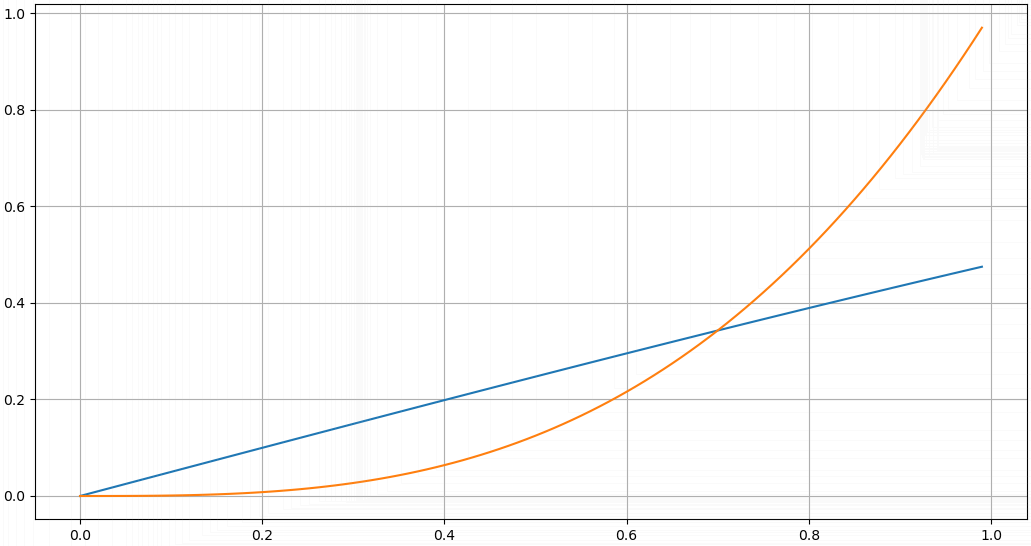
\includegraphics[scale=0.4]{7a.png}
\end{center}
Utifra grafen ser løsningen ut til å være cirka $x = 0,7$

Verdiene for $f$ og $g$ kan eventuelt sammenlignes over punktene i x-aksen for å finne x-verdien der de skjærer:
\begin{lstlisting}
skjaeringspunkter = [round(x, 2) for x in x_akse if abs(f(x) - g(x)) < 0.001]
\end{lstlisting}

\opgd{b}
\lstinputlisting[language=Python]{7b.py}

\opgd{c}
\lstinputlisting[language=Python]{7c.py}
\end{enumerate}

\newpage
\opg{7}
\begin{enumerate}[leftmargin=*,itemsep=0.75cm,labelsep=1.5em,label=\alph*)]
\opgd{d}
\lstinputlisting[language=Python]{7d.py}
Gir løsningen "Halveringsmetoden ga resultatet x = 0.6999 (etter 10 iterasjoner)"
\end{enumerate}

% % % % % % % % % % % % % % % % % % % % % % % % % % % % % % % % % % % % % % % % 

\end{document}
